\chapter{Perancangan}
\label{sec:perancangan}

Bab ini membahas mengenai perancangan aplikasi yang akan dibangun meliputi diagram kelas rinci beserta deskripsi dan fungsinya.

\section{Rancangan Kelas Lengkap}
\label{sec:kelaslengkap}
Rancangan kelas dibawah ini akan menampilkan keseluruhan kelas yang akan digunakan. Deskripsi kelas berserta fungsi dari diagram kelas tersebut adalah sebagai berikut:

\begin{figure}[H]
	\centering  
	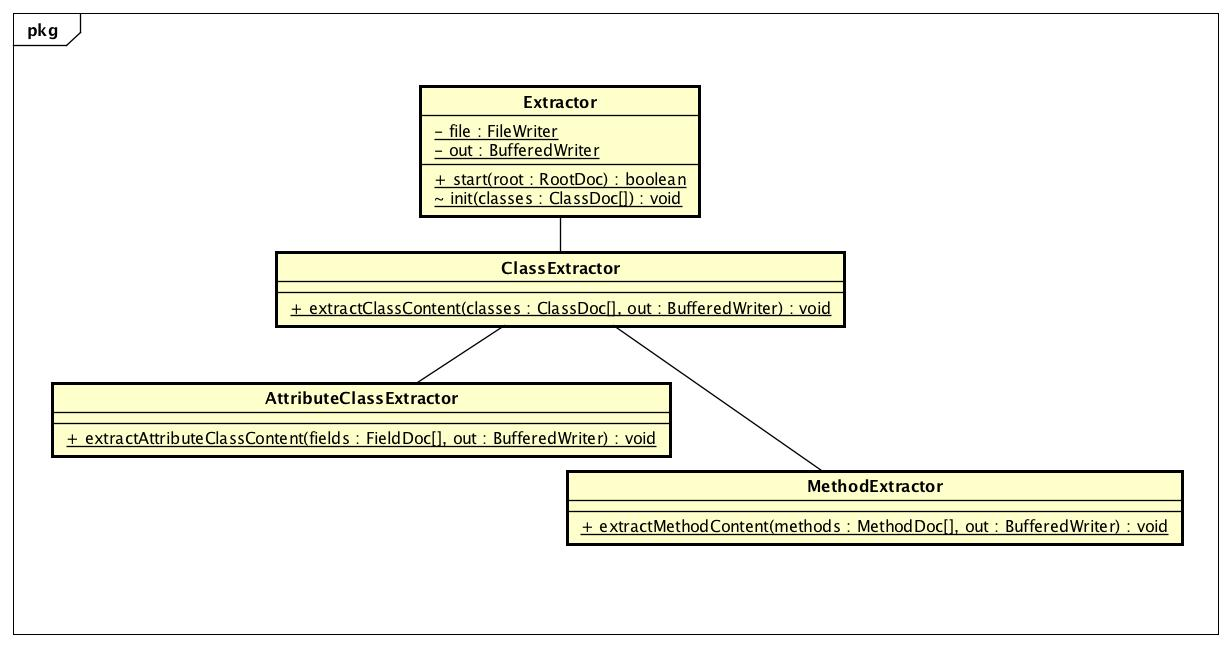
\includegraphics[scale=0.38]{kelas-diagram}  
	\caption[Kelas Diagram]{Kelas Diagram} 
	\label{fig:kelas-diagram} 
\end{figure} 

\begin{enumerate}
	\item {\texttt{Extractor}}\\
	Kelas ini merupakan kelas untuk menjalan {\it custom doclet}. Kelas ini memiliki 2 atribut yaitu sebagai berikut:
	\begin{itemize}
		\item \texttt{FileWriter file} - turuan dari kelas \texttt{OutputStreamWriter} yang digunakan untuk menulis kedalam sebuah {\it file}.
		\item \texttt{BufferedWriter out} - turunan dari kelas \texttt{Writer} yang digunakan untuk menulis file text.
	\end{itemize}
	Kelas ini memiliki {\it method} sebagai berikut:
	\begin{itemize}
		\item \texttt{start}\\
		{\it Method} ini berperan sebagai {\it method} untuk menjalankan {\it custom doclet}\\
		\textbf{Parameter:}
		\begin{itemize}
			\item \texttt{RootDoc root} - objek RootDoc yang berperan sebagai mengambil seluruh informasi spesifik dari {\it option} yang terdapat pada {\it command-line} sebuah {\it terminal}. Selain itu berperan juga untuk mengambil informasi dari sekumpulan file {\it java} yang akan di proses.
		\end{itemize}
		\item \texttt{init}\\
		{\it Method} ini berperan untuk menulis kedalam sebuah {\it file} saat javadoc berjalan.\\
		\textbf{Parameter:}
		\begin{itemize}
			\item \texttt{ClassDoc[] classes} - sebuah array yang berisikan sekumpulan {\it file java} yang akan di proses.
		\end{itemize}
	\end{itemize}

	\item {\texttt{ClassExtractor}}\\
	Kelas ini merupakan kelas untuk mengambil informasi dari sebuah kelas. Kelas ini memiliki {\it method} sebagai berikut:
	\begin{itemize}
		\item \texttt{extractClassContent}\\
		{\it Method} ini akan menampilkan nama kelas berserta penjelasan dari kelas tersebut. Didalam {\it method} ini akan memanggil {\it method} \texttt{extractAttributeClassContent} dan \texttt{extractMethodContent}\\
		\textbf{Parameter:}
		\begin{itemize}
			\item \texttt{ClassDoc[] classes} - sebuah array berisikan sejumlah kelas
			\item \texttt{BufferedWriter out} - turunan dari kelas \texttt{Writer} yang digunakan untuk menulis file text.
		\end{itemize}
	\end{itemize}
		 
	\item {\texttt{AttributeClassExtractor}}\\
	Kelas ini merupakan kelas untuk mengambil informasi sebuah atribut yang terdapat pada kelas. Kelas ini memiliki {\it method} sebagai berikut:
	\begin{itemize}
		\item \texttt{extractAttributeClassContent}\\
		{\it Method} ini akan menampilkan atribut-atribut yang dimiliki oleh sebuah kelas.\\
		\textbf{Parameter:}\\
		\begin{itemize}
			\item \texttt{FieldDoc[] fields} - sebuah array berisikan sejumlah atribut dari kelas
			\item \texttt{BufferedWriter out} - turunan dari kelas \texttt{Writer} yang digunakan untuk menulis file text.
		\end{itemize}
	\end{itemize}

	
	\item {\texttt{MethodExtractor}}\\
	Kelas ini merupakan kelas untuk mengambil informasi sebuah {\it method} terdapat pada kelas. Kelas ini memiliki {\it method} sebagai berikut:
	\begin{itemize}
		\item \texttt{extractMethodContent}\\
		{\it Method} ini akan menampilkan {\it method-method} yang dimiliki oleh sebuah kelas.\\
		\textbf{Parameter:}
		\begin{itemize}
			\item \texttt{ClassDoc superclass} - sebuah objek ClassDoc
			\item \texttt{MethodDoc[] methods} - sebuah array berisikan sejumlah {\it method} dari kelas
			\item \texttt{BufferedWriter out} - turunan dari kelas \texttt{Writer} yang digunakan untuk menulis file text.
		\end{itemize}
	\end{itemize}
	
\end{enumerate}

\section{Rancangan Antarmuka}
\label{sec:antarmuka}
Rancangan antarmuka perangkat lunak yang dibuat adalah melalui sebuah {\it terminal} pada {\it Linux} dan {\it command prompt} pada {\it Windows}. Berikut adalah antarmuka jika menggunakan {\it terminal} pada {\it Linux}: 

\begin{figure}[H]
	\centering  
	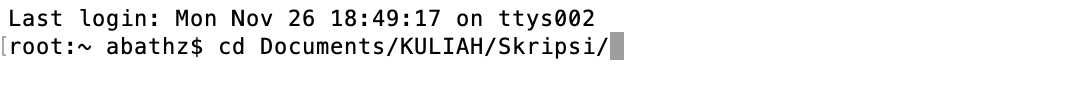
\includegraphics[scale=0.5]{1}  
	\caption[Kelas Diagram]{Mengarahkan kedalam folder dari perangkat lunak} 
	\label{fig:1} 
\end{figure}
Langkah pertama adalah berpindah dari direktori awal ke direktori perangkat lunak yang dibuat. Untuk berpindah direktori perlukan {\it command} \texttt{cd} atau kepanjangan dari {\it change directory} lalu diikuti dengan lokasi direktori yang diinginkan. Pada gambar \ref{fig:1} direktori perangkat lunak terdapat di dalam folder Document lalu folder KULIAH lalu folder Skripsi dan terakhir folder javadoc-to-latex kemudian tekan tombol {\it enter} lalu direktori akan langsung berpindah ke direktori yang dituju.

\begin{figure}[H]
	\centering  
	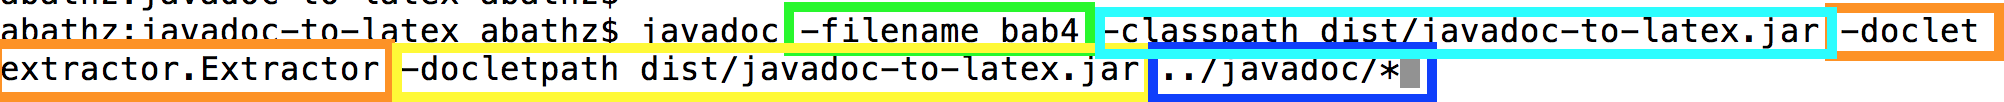
\includegraphics[scale=0.5]{2}  
	\caption[Kelas Diagram]{Kelas Diagram} 
	\label{fig:2} 
\end{figure}
Langkah kedua adalah menjalan perangkat lunak yang dibuat. Diawali dengan command \texttt{javadoc} lalu dikuti 3 buah argumen. Argumen pertama(jingga) adalah sebuah kelas untuk menjalankan {\it custom doclet} dari perangkat lunak yang dibuat. Argumen pertama tersebut akan menjalankan kelas bernama \texttt{Extractor} yang terdapat didalam {\it package} \texttt{extractor}. Kemudian argumen kedua(kuning) adalah {\it custom doclet} yang berperan untuk mengambil informasi kelas, atribut, {\it method} dari sekumpulan {\it file java} dan argumen ketiga(biru) adalah lokasi sekumpulan {\it file java} yang akan diproses. Pada gambar \ref{fig:2}, lokasi {\it file-file} tersebut terdapat pada folder javadoc. Folder javadoc tersebut berada direktori folder Skripsi.

\begin{figure}[H]
	\centering  
	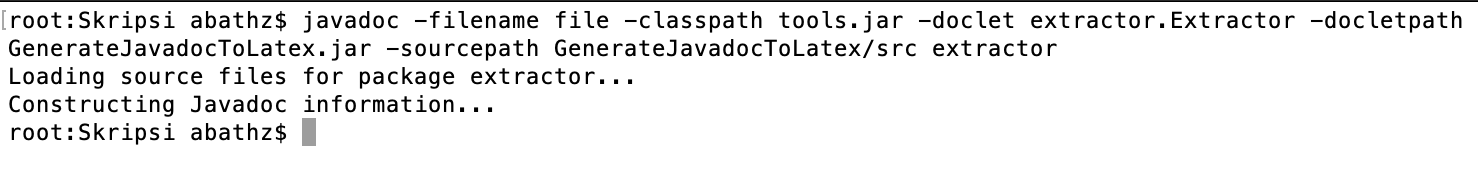
\includegraphics[scale=0.5]{3}  
	\caption[Kelas Diagram]{Kelas Diagram} 
	\label{fig:3} 
\end{figure}
Perangkat lunak yang dibuat akan membaca seluruh isi folder yang dituju, pada contoh gambar \ref{fig:3}, terdapat 5 {\it file java} yang terdapat didalam folder javadoc. Lalu perangkat lunak akan melakukan ekstrasi informasi terhadap masing-masing {\it file} tersebut. Jika proses ekstraksi selesai maka proses berhenti.
























